\documentclass[border=0.2ex,svgnames,tikz]{standalone}
\usepackage{fontspec}
\setmainfont{Source Serif 4}
\setsansfont{Source Sans 3}
\setmonofont{Source Code Pro}
\usepackage{ctex}
\setCJKmainfont[BoldFont=Source Han Sans CN]{Source Han Serif CN}

\usetikzlibrary{trees, positioning, shadows}

\begin{document}
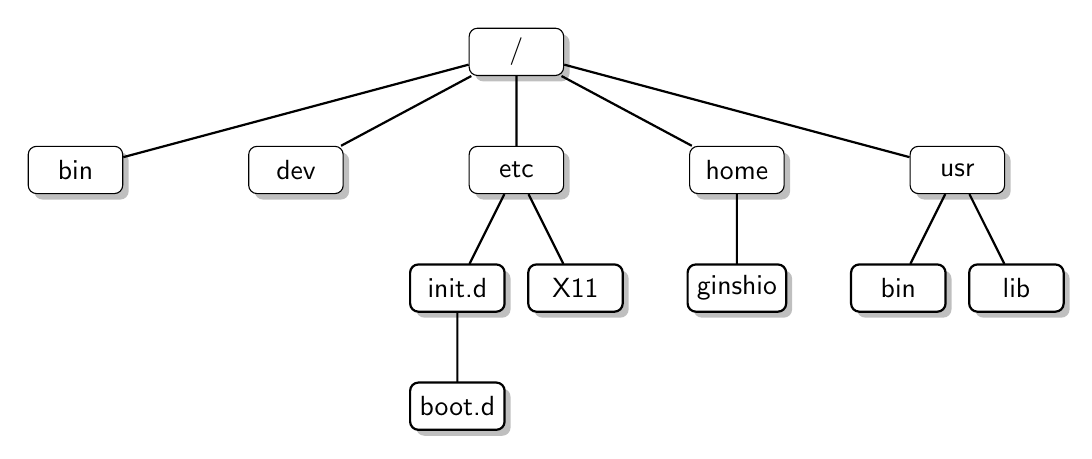
\begin{tikzpicture}[
    font=\sffamily,
    edge from parent/.style={draw, thick},
    every node/.style={draw, rectangle, rounded corners=3pt, fill=white, drop shadow, minimum width=1.2cm, minimum height=0.6cm, align=center},
    level 1/.style={sibling distance=2.8cm},
    level 2/.style={sibling distance=1.5cm},
    level distance=1.5cm
  ]

  \node {/}
    child { node {bin} }
    child { node {dev} }
    child { node {etc}
      child { node {init.d}
        child { node {boot.d} }
      }
      child { node {X11} }
    }
    child { node {home}
      child { node {ginshio} }
    }
    child { node {usr}
      child { node {bin} }
      child { node {lib} }
    };

\end{tikzpicture}
\end{document}
